\chapter{Implementation}
\label{ch:implementation}
\section{Introduction}
This chapter describes the planning and implementation phases.

\section{Software Development Methodology}
\subsection{Waterfall Model}
\subsection{}

\section{Planning}
As the timeline of the project is restricted and has a fixed deadline, it is important that the project is planned carefully in order to deliver a complete solution.

Gantt


\section{Version Control}
Git - branches

\section{Dependency Management}

\section{Implementation Process}
Following the Gantt chart, ...

\subsection{Initialisation}
The first step of the implementation was to initialise a Git repository and a Java environment with Maven dependency management. Since the project would depend on many libraries for displaying and processing data, Maven is able to manage versioning and interdependencies of these libraries.

\subsection{Program AB}
As a result of the research in earlier phases, it was decided that this system would use a rule-based chatbot architecture, namely AIML as it is widely used in current chatbot systems. Program AB is a Java implementation of AIML 2.0 provided by ALICE A.I. Foundation \cite{programab_2013}. While this repository is no longer being developed, the choice for this project was to use a fork of this source, which is provided as a Maven dependency \cite{lumenrobot2016}.

Once the Maven dependency had been loaded into the project's {\it{pom.xml}} file, I was able to experiment with the chatbot. The {\it{program-ab}} source contains the original AIML implementation of a bot named S.U.P.E.R. created by \citeauthor{wallace2009anatomy}, which gives examples of the many elements of the AIML style.

An initial program was written for experimenting with AIML and the example bot, as seen in Figure~\ref{fig:super}. 

\begin{figure}[ht]
	\centering
	\subfloat[Initial code]{{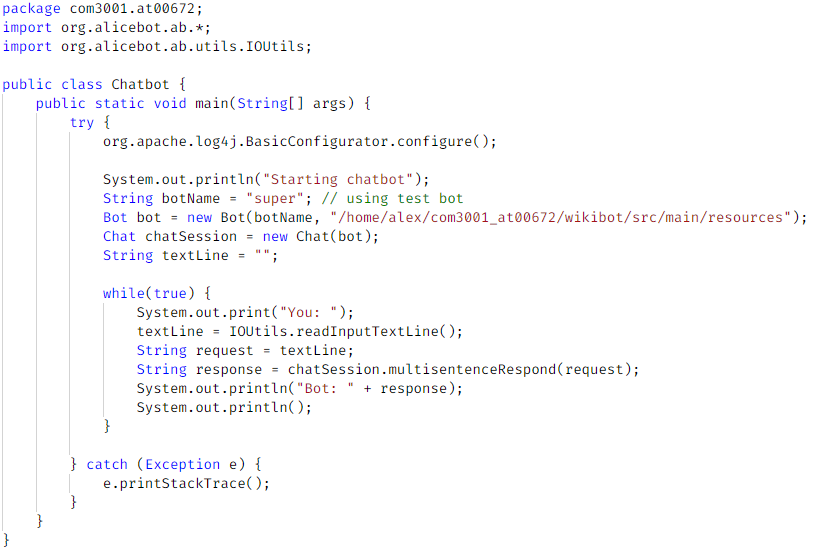
\includegraphics[width=12cm]{code1} }}%
	\qquad
	\subfloat[Chatting with S.U.P.E.R.]{{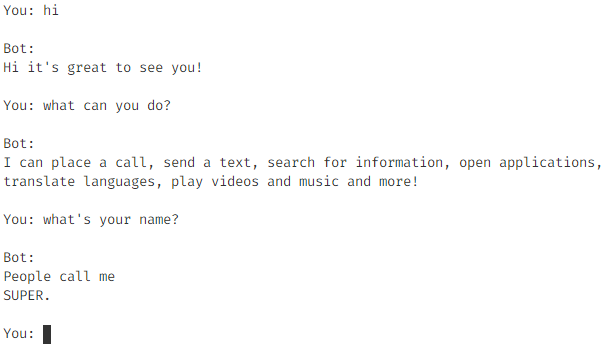
\includegraphics[width=12cm]{super} }}%	
	\caption{Initial chatbot interactions}
	\label{fig:super}
\end{figure}

\newpage
Having experimented with the example chatbot, my next task was to initialise my own chatbot. The Program AB Bot has a number of functions to load its required files from a directory. The file structure is as follows:

\begin{outline}
	\1 \textbf{bots} The parent bots directory
		\2 \textbf{\emph{botName}} The name of the bot
			\3 \textbf{aiml} The AIML pattern files 
			\3 \textbf{aimlif} AIML Intermediate Format files which are generated by the Bot
			\3 \textbf{config} Configuration files
			\3 \textbf{maps} Map files
			\3 \textbf{sets} Set files
\end{outline}
	
Once the structure was initialised, a file was created named {\it{conversation.aiml}}, which contained the first AIML patterns for conversing with the chatbot. The contents of this file are shown in Figure~\ref{fig:aiml1}. Some of the key features here are the use for the {\it{<srai>}} tag on line 17, which is a powerful function for resolving synonyms here. This allows us to route the input of 'hi' to the 'hello' pattern. This saves us repeating several lines of code, and is used heavily later in the project. Also, in lines 4 and 15 we are using wildcard symbols. This allows us to match zero or more words, and these can then be passed into other parts of the conversation. In AIML, the following wildcards can be used:

\begin{itemize}
	\item \# matches zero or more words (higher priority)
	\item \_ matches one or more words (higher priority)
	\item \^{} matches zero or more words (lower priority)
	\item * matches one or more words (lower priority)
\end{itemize}

So in our `hello' example, the given pattern will match any of the following inputs: `Hello', `Hello there', `Hi bot', `Hi', `Hi there'. It will not, however, match an input such as `Why hello there', because we have not told the bot how to divide that given input; nor does the bot recognise `good afternoon' and so on.

\begin{figure}[h]
	\centering
	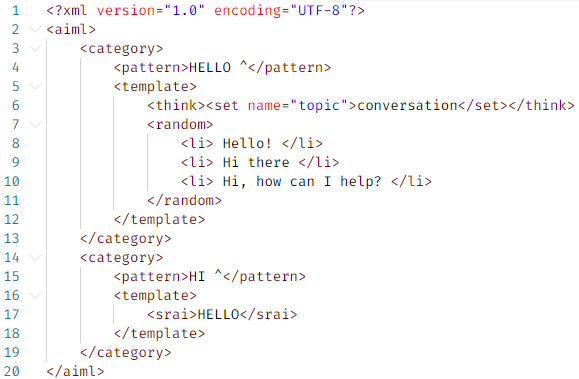
\includegraphics[width=.5\paperwidth]{aiml1}
	\caption{Initial AIML configuration}
	\label{fig:aiml1}
\end{figure}

\newpage
\subsection{DBPedia}
Now that the basic chatbot system has been set up, we need to provide functionality to the system by querying our datasource. DBPedia was selected based on the research in Section~\ref{sec:dbpedia}, because it provides an organised dataset from Wikipedia articles. It can be queried via a SPARQL endpoint, and returns data in an RDF format, which can be processed by our system.

There are a number of online resources which allow us to experiment with querying DBPedia. My preferred resource is SPARQL Explorer \footnote{http://dbpedia.org/snorql/}, which allows us to write queries and see the result in several formats, including a tabular format. For example, if we want to find musicians born in Manchester, we can construct the following SPARQL query:
\begin{figure}[h]
	\begin{lstlisting}
		SELECT ?person ?birthPlace ?name
		WHERE {
		  ?person a dbo:MusicalArtist .
		  ?person rdfs:label ?name .
		  ?person dbo:birthPlace ?birthPlace .
		  filter(?birthPlace = dbr:Manchester)
		  filter(langMatches(lang(?name), 'en'))
		} LIMIT 50 
	\end{lstlisting}
	\caption{An example SPARQL query}
	\label{fig:sparql}
\end{figure}

Executing this query returns a list of the first 50 results of musicians born in Manchester, as shown in Figure~\ref{fig:sparql1}. The format of SPARQL queries has some similarities with SQL queries, using keywords such as SELECT and WHERE. In this query, we are filtering to find each person that has the property {\it{dbo:MusicalArtist}}, which is shorthand for {\it{\url{http://dbpedia.org/ontology/MusicalArtist}}} which references the DBPedia ontology. We are setting the variable {\it{?name}} to the property {\it{rdfs:label}} which contains the name attribute of the person; the same applies for {\it{dbo:birthPlace}} references their birth place. Finally, we are filtering the results. First, we are filtering the results to only musicians whose birth place is Manchester. Secondly, we are filtering the {\it{?name}} results by language, to remove any duplicate results where the name is given in multiple languages.

\begin{figure}[h]
	\centering
	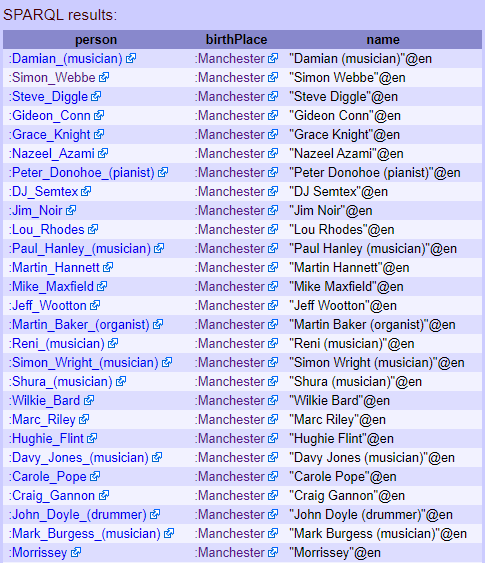
\includegraphics[width=8cm]{snorql}
	\caption{SPARQL query results}
	\label{fig:sparql2}
\end{figure}

In our Java system, these queries have to be constructed and executed programmatically, based on the user's input. For executing SPARQL queries, Apache Jena \cite{apachejena} provides RDF functionality for querying an RDF model. To test this, the Apache Jena dependencies are loaded into our Maven dependency file. This allows us to utilise the {\it{org.apache.jena}} libraries to query the endpoint. To test the connection, a function was written to test the DBPedia endpoint, as shown in Figure~\ref{fig:testrdf}.

\begin{figure}[h]
	\centering
	\subfloat[Test connection code]{{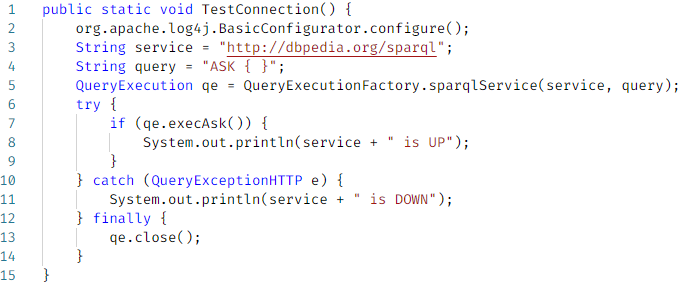
\includegraphics[width=.45\textwidth]{testrdf} }}%
	\qquad
	\subfloat[Successful result]{{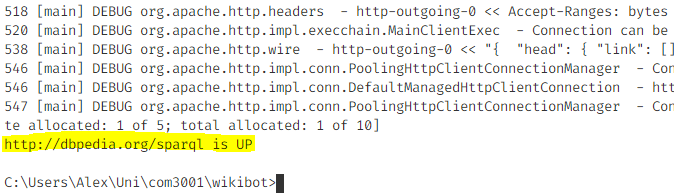
\includegraphics[width=.45\textwidth]{testrdf2} }}%
	\caption{Testing the SPARQL Endpoint}
	\label{fig:testrdf}
\end{figure}

For executing and processing more functional queries, we have to first generate a query string. As an example, we will use the query we saw in Figure~\ref{fig:sparql}. Once the query has been executed, we have to loop through the results and do some processing, such as printing to the console. The process for this is shown in Figure~\ref{fig:querysparql}. Here, our query string requires the {\it{PREFIX}} keyword to define the names of the prefixes for the ontologies we are using. The result from this execution exactly matches the result from the experimentation in Figure~\ref{fig:sparql2}.

\begin{figure}[h]
	\centering
	\subfloat[Testing query code]{{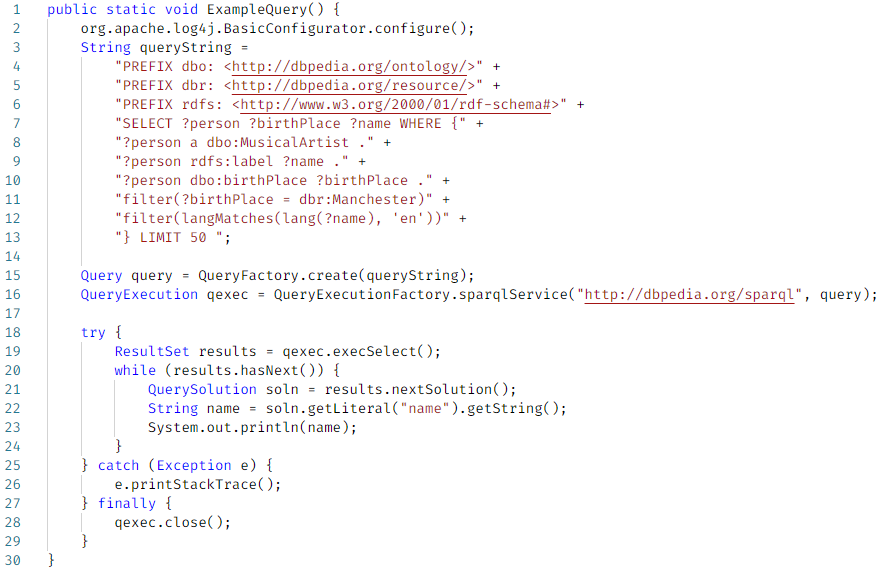
\includegraphics[width=.70\textwidth]{sparql1} }}%
	\qquad
	\subfloat[Result]{{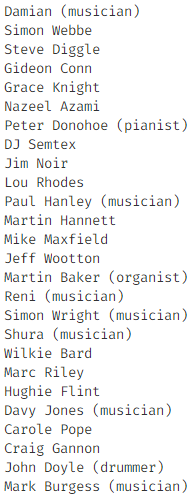
\includegraphics[width=.20\textwidth]{sparql2} }}%
	\caption{Querying the SPARQL endpoint}
	\label{fig:querysparql}
\end{figure}

\subsection{Linking the Chatbot}
Now that we have a basis for querying the DBPedia dataset, the chatbot now has to be able to query the endpoint. For this we need to implement the following:
\begin{enumerate}
	\item AIML patterns to match user input to a query
	\item A query builder to convert the user input into a SPARQL query
	\item A service to execute the function and process the results
\end{enumerate}
The next sections explain how these were implemented and connected in the final system to achieve the required functionality.

\subsubsection{AIML Patterns}
One of the key functions of this chatbot is to match input patterns to desired queries. There are a number of challenges that arise here. Firstly, a query can be asked in many different ways. For example, to find out the date of birth of a person, a user may ask: {\it`What is *'s' birthdate?', `When was * born?', `* birth date', `Tell me when * was born'}. The bot must then distinguish between these queries and `how old is *' as those are two distinct functions.

Furthermore, one of the requirements of the system is that is can deal with pronouns and maintain context. As such, the user should be able to ask follow-up questions by continuing a conversation, e.g. {\it `When was he born?'} - the chatbot must remember who {\it `he'} is, and if that is not known, the chatbot must ask for more information to continue the query.

\subsubsection{Query Builder}

\subsubsection{DBPedia Service}

\subsection{Web Interface}

\subsection{Hibernate Database}


\newpage
\section{Challenges}
\subsection{Spring Framework}

\subsection{Dataset Inconsistencies}
\begin{itemize}
	\item Actors 
	\item Countries - England displayed as a dbo:MusicalArtist
\end{itemize}

\subsection{Limitations of AIML}
Regex
Pattern matching - rule-based - synonyms

\subsection{SPARQL Queries}
\begin{itemize}
	\item Searching
	\item Lists - return order - vrank
\end{itemize}
\section{Conclusion}


